\chapter{离散数学}
\section{图论}

\noindent 警察抓强盗的问题 (Cops and Robber Problem)

有一个图, 警察位于一个节点上, 强盗可以选择初始节点, 之后警察和强盗轮流在图上移动, 可以从一个节点走到邻接的节点, 也可以原地不动. 如果警察一定能抓到强盗, 则称这个图是警察必胜的, 反之称为强盗必胜的. 给定一个图, 判断是警察必胜还是强盗必胜.

~

定义一类节点为陷阱点如下: 

如果一个节点 $ P $ 与一个节点 $ A $ 邻接, 且 $ P $ 的其他所有邻居都和 $ A $ 邻接, 则称 $ P $ 是一个陷阱节点 ( Pitfall ), 含义是只要强盗在 $ P $ 点而警察在 $ A $ 点时, 警察就获胜了. 这里 $ A $ 点称为攻击点 ( Attack ).

引理: 如果图中存在一个陷阱节点, 则可以去掉这个节点和它关联的边, 不影响警察和强盗的输赢.

\begin{figure*}[htbp]
\centering
 \begin{tabular}{c @{\hspace{.2\textwidth}} c}
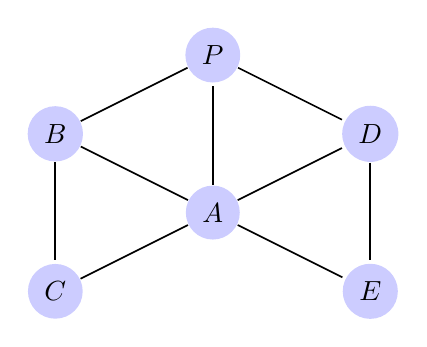
\begin{tikzpicture}[> = stealth, % arrow head style
	shorten > = 1pt, % don't touch arrow head to node
	auto,
	node distance = 3cm, % distance between nodes
	semithick % line style
	,auto=left,every node/.style={circle,fill=blue!20}]
	\node (n1) at (-2,1.)		{$B$};
	\node (n2) at (-2,-1.)  	{$C$};
	\node (n3) at (2,1.) 	{$D$};
	\node (n4) at (2,-1) 	{$E$};
	\node (n5) at (0,0) 	{$A$};
	\node (n6) at (0,2)	{$P$};
	\draw (n1)--(n2);
	\draw (n3)--(n4);
	\draw (n1)--(n5) -- (n4);
	\draw (n2)--(n5) -- (n3);
	\draw (n1)--(n6) -- (n3);
	\draw (n5)--(n6);

	%\draw [red,very thick](n4)--(n5);
	%\draw [red,very thick] (n1) .. controls (-2,-2.5)  ..(n4);
	%\draw [red,very thick](n1) .. controls (2,-3.5) 	..(n5);
\end{tikzpicture} & 
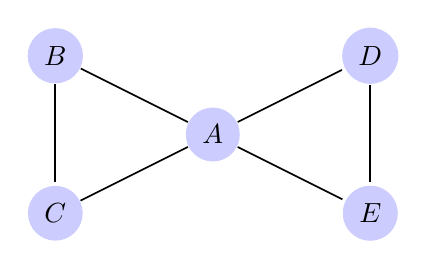
\begin{tikzpicture}[> = stealth, % arrow head style
	shorten > = 1pt, % don't touch arrow head to node
	auto,
	node distance = 3cm, % distance between nodes
	semithick % line style
	,auto=left,every node/.style={circle,fill=blue!20}]
	\node (n1) at (-2,1.)		{$B$};
	\node (n2) at (-2,-1.)  	{$C$};
	\node (n3) at (2,1.) 	{$D$};
	\node (n4) at (2,-1) 	{$E$};
	\node (n5) at (0,0) 	{$A$};
	\draw (n1)--(n2);
	\draw (n3)--(n4);
	\draw (n1)--(n5) -- (n4);
	\draw (n2)--(n5) -- (n3);
\end{tikzpicture}
 \\
$ G $ & $ H $
\end{tabular}

\end{figure*}

证明: 假设原图是 $ G $, 有一个陷阱节点 $ P $ 和攻击点 $ A $, 移除陷阱节点 $ P $ 和其相连的边之后得到的图为 $ H $. 如果 $ H $ 是警察必胜的, 则在 $ G $ 中警察也必胜, 原因是在 $ G $ 中警察可以复制 $ H $ 中的策略, 当强盗位于 $ P $ 点时, 注意到无论下一步强盗走到哪个节点, 或者不动, 都可以在 $ A $ 点一步到达, 对于警察来说, 强盗位于 $ P $ 点就像位于 $ A $ 点一样, 所以警察沿用原来的策略以 $ A $ 点为目标即可. 反过来如果强盗在 $ G $ 中必胜, 则他在 $ H $ 中也必胜. 

另一方面, 如果强盗在 $ H $ 中必胜, 也是同样的道理, 在 $ G $ 中, 当警察位于点 $ P $ 时, 强盗可以当做警察在
$ A $ 点一样按原来的策略逃脱. 这一条的对偶命题同样成立: 如果警察在 $ G $ 中必胜, 则在 $ H $ 中也必胜.

以上证明了一个图去掉一个陷阱节点后与原图是等价的. 这样可以不断去掉陷阱节点, 直到不能去掉为止. 如果最终剩余一个节点, 则警察必胜. 否则强盗必胜.

\newpage

%------------------------------------------------------------------------------%
